\section{Partitioning a Path}
\label{sec:path}

In this section we present an optimal algorithm to perform
parametric search on a graph that is a path of $n$ vertices. 
The algorithm follows the paradigm of parametric search by repeatedly performing 
feasibility tests over potential optimal values, as it gathers 
information so that subsequent feasibility tests can be 
performed increasingly faster. The improvement in speed of the subsequent 
feasibility tests is enough so that the entire running time is linear.
Our discussion focuses on the max-min problem;
at the end of the section we identify the changes necessary
for the min-max problem.
Throughout this section we assume that the vertices of any path or subpath
are indexed in increasing order from the start to the end of the path.

We first consider the running time of {\it PATH0},
to determine how the approach might be accelerated.
All activities except for feasibility testing use a total of $O(n)$ time.
Feasibility testing can use a total of $\Theta (n \log n)$ time in the worst case,
since there will be $\Theta (\log n)$ values to be tested in the worst case,
and each feasibility test takes $\Theta (n)$ time.
It seems unlikely that one can reduce the number of tests that need to be made,
so then to design a linear-time algorithm,
it seems necessary to design a feasibility test that will quickly begin to take $o(n)$ time.
We show how to realize such an approach.

We shall represent the path by a partition into subpaths, each of which can be searched in time proportional to the logarithm of its length. 
Each such subpath will possess a property
that makes feasibility testing easier.
Either the subpath will be singular or resolved.
A subpath $P'$ is {\it singular} if it consists of one vertex,
and it is {\it resolved} if no value in $M(P')$ falls in the interval
$(\lambda_1, \lambda_2 )$.
If a subpath is resolved,
then the position of any one cut determines the positions
of all other cuts in the subpath,
irrespective of what value of $\lambda$ we choose from within
$(\lambda_1, \lambda_2 )$.
If we have arranged suitable data structures when the subpath becomes resolved,
then we do not need a linear scan of it.

To make the representation simple, we restrict the subpaths in the partition to have lengths that are powers of 2.
Each subpath will consist of vertices whose indices are
$(j-1)2^i+1, \ldots ,j\:2^i$ for integers $j>0$ and $i \geq 0$.
Initially the partition will consist of $n$ singular subpaths.
Each nonsingular subpath will have $i>0$.
When introduced into the partition,
each such subpath will replace its two {\it constituent subpaths},
the first with indices $(2j-2)2^{i-1}+1, \ldots ,(2j-1)2^{i-1}$,
and the second with indices $(2j-1)2^{i-1}+1, \ldots ,(2j)2^{i-1}$.

We represent the partition of path $P$ into the subpaths with 
three arrays $last[1..n]$, $ncut[1..n]$ and $next[1..n]$. 
Consider any subpath in the partition,
with first vertex $v_f$ and last vertex $v_t$.
Let $v_l$ be an arbitrary vertex in the subpath.
The array $last$ identifies the end of a subpath,
given the first vertex of a subpath.
Thus $last(l)=t$ if $l=f$ and is arbitrary otherwise.
Given a cut on the subpath,
the array $next$ identifies,
in constant time, a cut further on in that subpath.
The array $ncut$ identifies the number of cuts skipped
in moving to that further cut.
Let $w(l,t)$ be the sum of the weights of vertices $v_l$ through $v_t$.
If $w(l,t) < \lambda_2$,
then $next(l)=null$ and $ncut(l)=0$.
Otherwise, $next(l) \geq l$ is the index of the last vertex before a cut,
given that $l=1$ or $v_l$ is the first vertex after a cut.
Then $ncut(l)$ is the number of cuts after $v_l$ up to and including the one
following $v_{next(l)}$.
We assume that the last cut on a subpath will leave
a (possibly empty) subset of vertices of total weight less than $\lambda_2$.
(Note that the last cut on the path as a whole must then be ignored.)

Given the partition into subpaths, we describe feasibility test {\it FTEST1}.
Let $\lambda$ be the value to be tested,
with $\lambda_1 < \lambda < \lambda_2$.
For each subpath, we use binary search to find the first cut,
and then, follow $next$ pointers and add $ncut$ values to
identify the number of cuts on the subpath.
When we follow a path of $next$ pointers,
we will compress this path.
This turns out to be a key operation as we consider
subpath merging and its effect on feasibility testing.
(Note that the path compression makes
{\it FTEST1} a function with side effects.)\\

\sspace
\noindent
{\bf func} {\it FTEST1} ({\bf path} $P$, {\bf integer} $k$, {\bf real} $\lambda$){\vspace{.05in}\\
$\T $ $f \ASG 1$\\
$\T $ $numcut \ASG -1$; $remainder\ASG 0$\\
$\T $ $\WH$ $f \leq n$ $\DO$ /* search the next subpath: */\\
$\T \T $ $t \ASG last(f)$\\
$\T \T $ $\IF$ $remainder + w(f,t) < \lambda$\\
$\T \T $ $\TN$ $remainder \ASG remainder + w(f,t)$\\
$\T \T $ $\EL$ \\
$\T \T \T $ $numcut \ASG numcut+1$ \\
$\T \T \T $ Binary search for a smallest $r$ so that $w(f,r) + remainder \geq \lambda$. \\
$\T \T \T $ $\IF$ $r<t$ \\
$\T \T \T $ $\TN$ \\
$\T \T \T \T $ $(s,sumcut) \ASG$ {\it search\_next\_path} $(r,t)$\\
$\T \T \T \T $ $numcut \ASG numcut+sumcut$ \\
$\T \T \T \T $ {\it compress\_next\_path} $(r,s,t,sumcut)$ \\
$\T \T \T $ $\EI$  \\
$\T \T \T $ $remainder \ASG w(s+1,t)$ \\
$\T \T $ $\EI$  \\
$\T \T $ $f \ASG t+1$  \\
$\T $ $\EW$ \\
$\T $ $\IF$ $numcut \geq k$ $\TN$ {\bf return}(``$lower$'') $\EL$ {\bf return}(``$upper$'') $\EI$ \\
{\bf endfunc}
 
\bigskip
\noindent
{\it search\_next\_path} ({\bf vertex\_index} $l,t$)\vspace{.05in}\\
$\T $ $sumcut \ASG 0$ \\
$\T $ $\WH$ $l < t$ and $next(l+1) \neq null$ \\
$\T \T $ $sumcut \ASG sumcut+ncut(l+1)$ \\
$\T \T $ $l \ASG next(l+1)$ \\
$\T $ $\EW$ \\
$\T $ {\bf return}$(l,sumcut)$ 
 
\bigskip
\noindent
{\it compress\_next\_path} ({\bf vertex\_index} $l,s,t$, {\bf integer} $sumcut$)\vspace{.05in}\\
$\T $ $\WH$ $l < t$ and $next(l+1) \neq null$ \\
$\T \T $ $sumcut \ASG sumcut-ncut(l+1)$ \\
$\T \T $ $ncut(l+1) \ASG ncut(l+1)+sumcut$ \\
$\T \T $ $temp \ASG next(l+1)$ \\
$\T \T $ $next(l+1) \ASG s$ \\
$\T \T $ $l \ASG temp$ \\
$\T $ $\EW$  

\dspace
\bigskip

Use of this feasibility test by itself is not enough to guarantee
a quick reduction in the time for feasibility testing.
This is because there is no assurance that the interval
$(\lambda_1, \lambda_2)$ will be narrowed in a manner
that allows longer subpaths to quickly replace shorter subpaths
in the partition of path $P$.
To achieve this effect,
we reorganize the positive values from $M(P)$
into submatrices that correspond in a natural way to subpaths.
Furthermore, we associate synthetic weights with these submatrices
and use these weights in selecting the weighted median for testing.
The synthetic weights place a premium on resolving first the values from submatrices corresponding to short subpaths.
However, using synthetic weights could mean that we consider many values of small weight repeatedly, causing the total time for selection to exceed $\Theta (n)$.
To offset this effect, we also find the unweighted median, and test this value.
This approach guarantees that we discard at least half of the submatrices'
representatives on each iteration,
so that each submatrix inserted into $\cal M$ need be charged
only a constant for its share of the total work in
selecting values to test.

We now proceed to a broad description of {\it PATH1}.
The basic structure follows that of {\it PARAM\_SEARCH}, in that there will be the routines {\it PATH1\_init\_mat}, {\it PATH1\_test\_val}, and {\it PATH1\_update\_mat}. 
However, we will slip the set-up and manipulation
of the data structures for the subpaths into the routines
{\it PATH1\_init\_mat} and {\it PATH1\_update\_mat}.
Let $large(M)$ be the largest element in submatrix $M$,
and let $small(M)$ be the smallest element in $M$.\\
 
\sspace
\noindent
{\it PATH1\_init\_mat}:\vspace{.05in}\\
$\T $ Initialize $\cal M$ to be empty. \\
$\T $ Call {\it mats\_for\_path}$(P,1,n)$ to insert submatrices of $M(P)$ into $\cal M$. \\
$\T $ $\FO$ $l \ASG 1$ $\TO$ $n$ $\DO$ $last(l) \ASG l$; $next(l) \ASG 0$; $ncut(l) \ASG 0$ $\EF$
 
\bigskip
\noindent
{\it PATH1\_test\_val}:\vspace{.05in}\\
$\T $ $R \ASG \emptyset$ \\
$\T $ $\FO$ each $M$ in $\cal M$ $\DO$ \\
$\T \T $ $\IF$ $large(M) < \lambda_2$ \\
$\T \T $ $\TN$ Insert $large(M)$ into $R$ with synthetic weight $w(M)/4$. $\EI$ \\
$\T \T $ $\IF$ $small(M) > \lambda_1$ \\
$\T \T $ $\TN$ Insert $small(M)$ into $R$ with synthetic weight $w(M)/4$. $\EI$ \\
$\T $ $\EF$ \\
$\T$ Select the (synthetic) weighted median element $\lambda$ in $R$. \\
$\T$ $\IF$ {\it FTEST1}$(P,k,\lambda ) = ``lower$'' $\TN$ $\lambda_1 \ASG \lambda$ $\EL$ $\lambda_2 \ASG \lambda$ $\EI$ \\
$\T$ Remove from $R$ any values no longer in $(\lambda_1,\lambda_2)$. \\
$\T$ $\IF$ $R$ is not empty \\
$\T$ $\TN$ \\
$\T \T$ Select the unweighted median element $\lambda '$ in $R$. \\
$\T \T$ $\IF$ {\it FTEST1}$(P,k,\lambda ') = ``lower$'' $\TN$ $\lambda_1 \ASG \lambda '$ $\EL$ $\lambda_2 \ASG \lambda '$ $\EI$ \\
$\T$ $\EI$ 
 
\bigskip
\noindent
{\it PATH1\_update\_mat}:\vspace{.05in}\\
$\T $ $\WH$ there is an $M$ in $\cal M$ such that $small(M) \geq \lambda_2$ or $large(M) \leq \lambda_1$ \\
$\T \T $ or $small(M) \leq \lambda_1 \leq \lambda_2 \leq large(M)$ $\DO$ \\
$\T \T $ $\IF$ $small(M) \geq \lambda_2$ or $large(M) \leq \lambda_1$ \\
$\T \T $ $\TN$ \\
$\T \T \T $ Delete $M$ from $\cal M$. \\
$\T \T \T $ $\IF$ this is the last submatrix remaining for a subpath $P'$ \\
$\T \T \T $ $\TN$ $glue\_paths(P')$ \\
$\T \T \T $ $\EI$ \\
$\T \T $ $\EI$ \\
$\T \T $ $\IF$ $small(M) \leq \lambda_1$ and $large(M) \geq \lambda_2$ \\
$\T \T $ $\TN$ Split $M$ into four square submatrices, each of synthetic weight $w(M)/8$. \\
$\T \T $ $\EI$ \\
$\T $ $\EW$
 
\dspace
\bigskip

\begin{figure}[thb]
\begin{center}
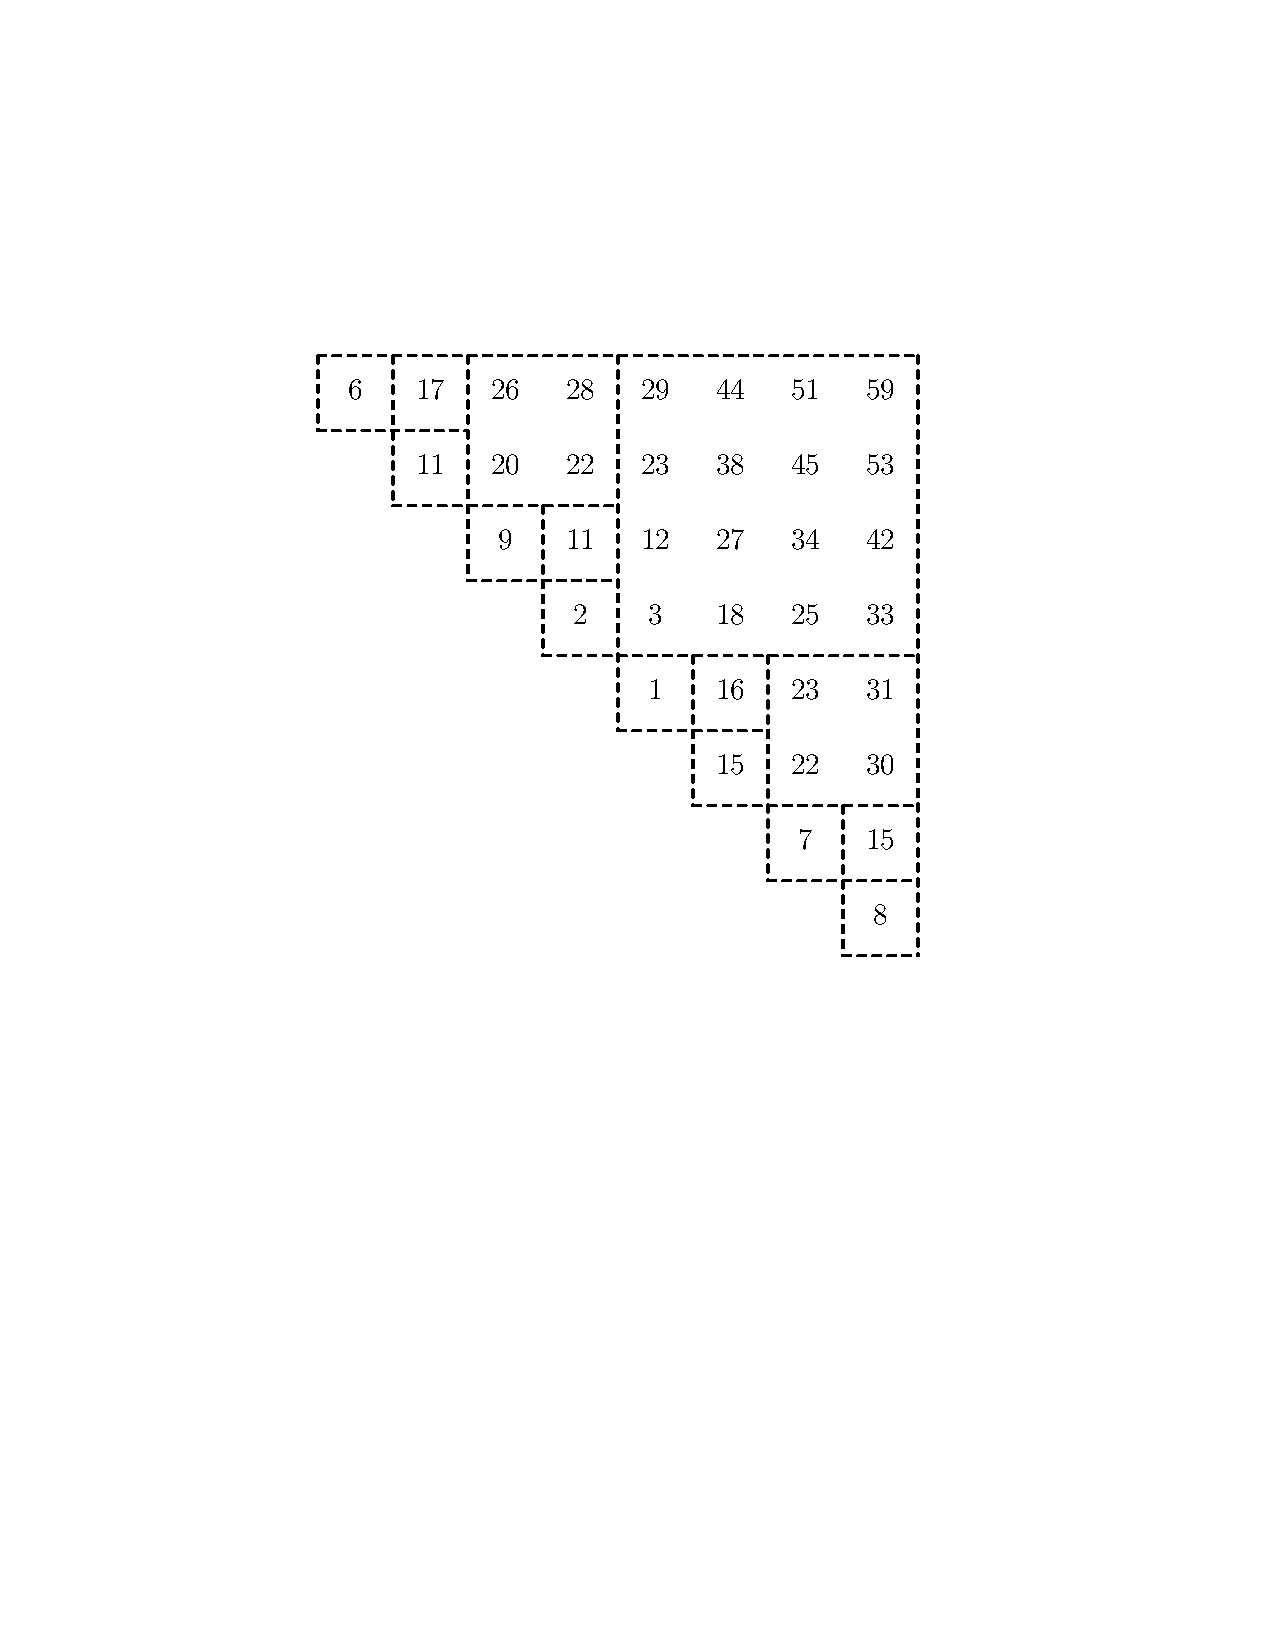
\includegraphics{fig3p1}
\end{center}
{\caption{\small Explicit representation of initial submatrices for $M(P)$ in {\it PATH1}}\label{fig3p1}}
\end{figure}

Below is the procedure {\it mats\_for\_path},
which inserts submatrices of the appropriate previously discussed synthetic weight into $\cal M$.
A call with arguments $f$ and $t$
will generate submatrices for all required subpaths of
a path containing the vertices with indices $f,f+1,\ldots ,t$.
(In this section, we assume that $f=1$ and $t=n$,
but we state the procedure in this form so that it can be used
in the next section too.)
The submatrices for the matrix $M(P)$ in Fig.~\ref{fig1}
are shown in Fig.~\ref{fig3p1}. 
Every subpath $P'$ that will appear in some partition of $P$
is initialized with $cleaned(P')$ and $glued(P')$ to {\bf false},
where $cleaned(P')$ indicates whether or not all values in
the submatrix associated with $P'$ are outside the interval
$(\lambda_1,\lambda_2)$,
and $glued(P')$ indicates whether or not all values in $M(P')$
are outside the interval $(\lambda_1,\lambda_2)$. \\

\sspace
\noindent
{\bf proc} {\it mats\_for\_path} ({\bf path} $P$, {\bf integer} $f,t$){\vspace{.05in}\\
$\T $ $size \ASG 1$ \\
$\T $ $w \ASG 4n^4$ /* synthetic weight for $1\times1$ submatrices */\\
$\T $ $\WH$ $f\leq t$ $\DO$ \\
$\T \T $ $\FO$ $i \ASG f$ $\TO$ $t$ $\BY$ $size$ $\DO$ \\
$\T \T \T $ Insert the succinct description of submatrix $[i\:..\:(i\!+\!\lceil size/2\rceil\!-\!1),$ \\
$\T \T \T \T $ $(i\!+\!\lceil size/2\rceil )..\:(i\!+\!size\!-\!1)]$ for $M(P)$ into $\cal M$ with synthetic weight $w$. \\
$\T \T \T $ Let $P'$ be the subpath of $P$ whose vertices have indices \\
$\T \T \T \T $ $i,\ldots ,i+size-1$. \\
$\T \T \T $ $cleaned(P') \ASG \FA$; $glued(P') \ASG \FA$ \\
$\T \T \T $ $\EF$ \\
$\T \T $ $size \ASG size*2$ \\
$\T \T $ $w \ASG w/2$ /* smaller synthetic weight for increased size of submatrix */\\
$\T \T $ $f \ASG size*\lceil (f-1)/size\rceil +1$ \\
$\T \T $ $t \ASG size*\lfloor t/size\rfloor$ \\
$\T $ $\EW$  \\
{\bf endproc}\\

\dspace
\bigskip

We next describe the procedure {\it glue\_paths}, which checks to see if two constituent subpaths can be combined together.
Let $P'$ be any subpath of weight at least $\lambda_2$, and let $f'$ and $t'$ be the indices of the first and last vertices in $P'$, resp.
Let the $\lambda$-{\it prefix} of $P'$, designated $\lambda${\it pref}$\,(P')$, be vertices $v_{f'},\cdots ,v_l$ in $P'$ where $l$ is the largest index such that $w(f',l) < \lambda_2$.
Let the $\lambda$-{\it suffix} of $P'$, designated $\lambda${\it suff}$\,(P')$, be vertices $v_l,\cdots ,v_{t'}$ in $P'$ where $l$ is the smallest index such that $w(l,t') < \lambda_2$. 
To glue two subpaths $P_2$ and $P_3$ together into a subpath $P_1$, we must have $(glued(P_2)$ {\bf and} $glued(P_3)$ {\bf and} $cleaned(P_1))$. 
Procedure {\it glue\_paths} sets the $next$ pointers from vertices in $\lambda${\it suff}$\,(P_2)$ to vertices in $\lambda${\it pref}$\,(P_3)$. \\

\sspace
\noindent
{\bf proc} {\it glue\_paths} ({\bf path} $P_1$){\vspace{.05in}\\
$\T $ $cleaned(P_1) \ASG \TR$\\
$\T $ $\IF$ $P_1$ has length 1\\
$\T $ $\TN$ \\
$\T \T $ $glued(P_1) \ASG \TR$ \\
$\T \T $ Let $l$ be the index of the vertex in $P_1$. \\
$\T \T $ $\IF$ $w(l,l) \geq \lambda_2$ $\TN$ $next(l) \ASG l$; $ncut(l) \ASG 1$ $\EI$ \\
$\T \T $ Reset $P_1$ to be subpath of which $P_1$ is now a constituent subpath. \\
$\T $ $\EI$ \\
$\T $ Let $P_2$ and $P_3$ be the constituent subpaths of $P_1$. \\
$\T $ $\WH$ $glued(P_2)$ and $glued(P_3)$ and $cleaned(P_1)$ and $P_1 \neq P$ $\DO$ \\
$\T \T $ $glued(P_1) \ASG \TR$\\
$\T \T $ Let $f_2$ and $t_2$ be resp. the indices of the first and last vertices in $P_2$. \\
$\T \T $ Let $f_3$ and $t_3$ be resp. the indices of the first and last vertices in $P_3$. \\
$\T \T $ $last(f_2) \ASG t_3$\\
$\T \T $ $\IF$ $w(f_2,t_3) \geq \lambda_2$\\
$\T \T $ $\TN$ \\
$\T \T \T $ $\IF$ $w(f_2,t_2) < \lambda_2$ \\
$\T \T \T $ $\TN$ $f \ASG f_2$ \\
$\T \T \T $ $\EL$ /* initialize $f$ to the front of $\lambda${\it suff}$\,(P_2)$ */ \\
$\T \T \T \T $ $f \ASG t_2$\\
$\T \T \T \T $ $\WH$ $w(f-1,t_2) < \lambda_2$ $\DO$ $f \ASG f-1$ $\EW$ \\
$\T \T \T $ $\EI$ \\
$\T \T \T $ $t \ASG f_3$ \\
$\T \T \T $ $\WH$ $f \leq t_2$ and $w(f,t_3) \geq \lambda_2$ $\DO$ \\
$\T \T \T $ /* set $next$ pointers for $\lambda${\it suff}$\,(P_2)$ */ \\
$\T \T \T \T $ $\WH$ $w(f,t) < \lambda_2$ $\DO$ $t \ASG t+1$ $\EW$ \\
$\T \T \T \T $ $ncut(f) \ASG 1$ \\
$\T \T \T \T $ $next(f) \ASG t$ \\
$\T \T \T \T $ $f \ASG f+1$ \\
$\T \T \T $ $\EW$ \\
$\T \T $ $\EI$  \\
$\T \T $ Reset $P_1$ to be subpath of which $P_1$ is now a constituent subpath. \\
$\T \T $ Let $P_2$ and $P_3$ be the constituent subpaths of $P_1$. \\
$\T $ $\EW$ \\
{\bf endproc}\\

\dspace

It would be nice if procedure {\it glue\_paths},
after setting pointers in $\lambda${\it suff}$\,(P_2)$,
would perform pointer jumping,
so that $next$ pointers for vertices in $\lambda${\it pref}$\,(P_1)$
would point to vertices in $\lambda${\it suff}$\,(P_1)$. 
Unfortunately, it is not apparent how to incorporate pointer jumping into {\it glue\_paths} without using $O(n)$ time over all calls in the worst case. 
%Unfortunately, it appears that requiring {\it glue\_paths}
%to perform such an activity would result in a total time
%over all calls of $O(n \log \log n)$ in the worst case.
%(We do not have a proof of this assertion,
%but extensive simulation seems to provide strong corroboration
%for such a conjecture.)
We thus opt for having {\it glue\_paths} do no pointer jumping,
and instead we do pointer jumping under the guise of path
compression in {\it FTEST1}.
We use an argument based on amortization to show that this works well.
\bigskip

\begin{lemma}
\label{lem:3:1}
Let $P$ be a path of $n$ vertices.
All calls to {\it glue-paths} will take amortized time of $O(n)$,
and {\it FTEST1} will search each subpath that is glued
in amortized time proportional to the logarithm of its length.
\end{lemma}
\begin{proof}
Suppose two subpaths $P_2$ and $P_3$ are glued together to give $P_1$,
where $P_1$ has weight at least $\lambda_2$.
We consider two cases.
First suppose either $P_2$ or $P_3$ has weight at most $\lambda_1$.
Let $P_m$ represent this subpath.
The time for {\it glue\_paths} is in worst case proportional
to the length of $P_m$.
Also, we leave a {\it glue-credit}
on each vertex in the $\lambda${\it pref}$\,(P_1)$ and $\lambda${\it suff}$\,(P_1)$,
and a {\it jump-credit} on each vertex in the $\lambda${\it pref}$\,(P_1)$.
The number of credits will be proportional to the length of $P_m$.
We charge this work and the credits to the vertices of $P_m$,
at a constant charge per vertex.
It is clear that any vertex in $P$ is charged at most once,
so that the total charge to vertices over all calls to {\it glue\_paths}
is $O(n)$.
The second case is when both $P_2$ and $P_3$ have weight at least $\lambda_2$.
In this case, the time for {\it glue\_paths} is proportional to the sum
of the lengths of $\lambda${\it suff}$\,(P_2)$
and $\lambda${\it pref}$\,(P_3)$,
and we use the glue-credits of $P_2$ and $P_3$ to pay for this.
The jump-credits are used by {\it FTEST1} rather than by {\it glue-paths},
and in fact, would present a problem if one tries to use them in {\it glue-paths}, as we discuss below.

Suppose both $P_2$ and $P_3$ have weight at least $\lambda_2$.
Then we might have wanted to have {\it glue-paths} jump the $next$ pointers
so that the $next$ pointer for a vertex in $\lambda${\it pref}$\,(P_2)$
would be reset to point to $\lambda${\it suff}$\,(P_3)$.
The time to reset such pointers would be proportional to the length
of $\lambda${\it pref}$\,(P_2)$.
The jump-credits of $\lambda${\it pref}$\,(P_3)$ could pay for this,
as long as the length of $\lambda${\it pref}$\,(P_2)$
is at most some constant (say 2)
times the length of the $\lambda${\it pref}$\,(P_3)$.
When the length of the $\lambda${\it pref}$\,(P_2)$
is at most twice the length of the $\lambda${\it pref}$\,(P_3)$,
we would not want to jump the pointers.

In general we could view a subpath as containing a sequence of
$\lambda$-{\it regions},
where each $\lambda$-region was once the $\lambda$-prefix of some subpath,
and the length of a $\lambda$-region is less than twice the length
of the preceding $\lambda$-region.
Note that the number of $\lambda$-regions in the sequence could be at most
the logarithm of the length of the subpath.
When gluing two subpaths together,
we could concatenate their sequences of $\lambda$-regions together,
and jump pointers over any $\lambda$-region that gets a predecessor
whose length is not more than twice its length.
Its jump-credits could then be used for this pointer jumping.
Searching a subpath in {\it FTEST1} would then take
time at most proportional to its length.

Of course {\it glue-paths} does not jump pointers.
However,
a lazy form of pointer-jumping is found in the path-compression of {\it FTEST1},
and the same sort of analysis can be seen to apply.
Suppose that {\it FTEST1} follows a pointer to a vertex
that was once in the $\lambda$-prefix of some subpath.
Consider the situation if {\it glue-paths} had jumped pointers.
If that pointer would have been present in the sequence of $\lambda$-regions,
then charge the operation of following that pointer to {\it FTEST1}.
Otherwise, charge the operation of following that pointer
to the jump-credits of the $\lambda$-prefix containing the vertex.
It follows that the number of pointers followed during a search
of a subpath that are not covered by jump-credits is at most
the logarithm of the length of the subpath.
Also, the binary search to find the position of the first cut
on a subpath uses time at most proportional
to the logarithm of the length of the subpath.
\end{proof}

\begin{lemma}
\label{lem:3:2}
Let $P$ be a path of $n$ vertices.
On the $i$-th iteration of the while-loop of {\it PATH1},
the amortized time used by feasibility test {\it FTEST1}
will be $O(i(5/6)^{i/5}\:n)$.
\end{lemma}

\begin{proof}
We first consider the synthetic weights assigned to submatrices in $\cal M$.
Corresponding to subpaths of lengths $1, 2, 4, \ldots , n$,
procedure {\it mats\_for\_path} creates
$n$ submatrices of size $1 \times 1$,
$n/2$ submatrices of size $1 \times 1$,
$n/4$ submatrices of size $2 \times 2$, and so on,
up through one submatrix of size $n/2 \times n/2$.
The total synthetic weight of the submatrices corresponding to each path length is
$4n^5, n^5, n^5/4, \ldots , 4n^3$, resp.
It follows that the total synthetic weight for submatrices of all path lengths is
less than $(4/3)*4n^5$.

Let $wgt(M)$ be the synthetic weight assigned to submatrix $M$.
Define the {\it effective weight},
denoted {\it eff\_wgt}$(M)$, of a submatrix $M$ in $\cal M$
to be $wgt(M)$ if both its smallest value and largest value
are contained in the interval $(\lambda_1, \lambda_2)$
and $(3/4)wgt(M)$ if only one of its smallest value and largest value
is contained in the interval $(\lambda_1, \lambda_2)$.
Let {\it eff\_wgt}$(\cal M )$ be the total effective weight of all submatrices in $\cal M$.
When a feasibility test renders a value (the smallest or largest)
from $M$ no longer in the interval $(\lambda_1, \lambda_2)$,
we argue that {\it eff\_wgt}$(M)$ is reduced by at least $wgt(M)/4$
because of that value.

If both values were contained in the interval $(\lambda_1, \lambda_2)$,
and one no longer is, then clearly our claim is true.
If only one value was contained in the interval $(\lambda_1, \lambda_2)$,
and it no longer is,
then $M$ is replaced by four submatrices of effective weights
$wgt(M)/8 + wgt(M)/8 + (3/4)wgt(M)/8 + (3/4)wgt(M)/8$ $< wgt(M)/2$,
so that there is a reduction in effective weight by greater than $wgt(M)/4$.
If both values were contained in the interval $(\lambda_1, \lambda_2)$,
and both are no longer in,
then we consider first one and then the other.
Thus every element that was in $(\lambda_1, \lambda_2)$ but no longer is
causes a decrease in {\it eff\_wgt}$(\cal M )$ by an amount
at least equal to its synthetic weight in $R$.
Values with at least half of the total weight in $R$
find themselves no longer in $(\lambda_1, \lambda_2)$.
Furthermore, the total weight of $R$ is at least $1/3$ of
{\it eff\_wgt}$(\cal M )$.
This follows since a submatrix $M$ has either two values in $R$
at a total of $2w(M)/4 = (1/2)w(M)$
or one value at a weight of $w(M)/4 = (1/3)(3w(M)/4)$.
Thus {\it eff\_wgt}$(\cal M )$
decreases by a factor of at least $(1/2)(1/3) = 1/6$ per iteration.

Corresponding to the subpaths of length $2^j$,
there are $n/2^j$ submatrices created by {\it mats\_for\_path}.
If such a matrix is quartered repeatedly until $1 \times 1$ submatrices result,
each such submatrix will have weight $n^4/2^{4j-2}$.
Thus when as little as $(n/2^j)*(n^4/2^{4j-2})$ synthetic weight remains,
all subpaths of length $2^j$ can still be unresolved.
This can be as late as iteration $i$,
where $i$ satisfies
$(4/3)*4n^5*(5/6)^i = n^5/2^{5j-2}$,
or $2^{5j}=(3/4)*(6/5)^i$.
While all subpaths of length $2^j$ can still be unresolved on this iteration,
at most $(1/2*1/2^4)^k = 1/2^{5k}$ of the subpaths of length $2^{j-k}$
can be unresolved for $k= 1, \ldots, j$.
Also, by Lemma~3.1, each subpath can be searched by {\it FTEST1}
in amortized time proportional to the logarithm of its length.
Thus the time to search path $P$ on iteration $i$ is at worst proportional to
$(j/2^j)n(1 + 1/2^5 + 1/2^{10} + \cdots )$,
which is $O((j/2^j)n)$.
From the relationship of $i$ and $j$,
$2^j = (3/4)^{1/5}(6/5)^{i/5}$,
and $j = (1/5)\log(3/4) + (i/5)\log (6/5)$.
The lemma then follows.
\end{proof}

\begin{lemma}
\label{lem:3:3}
The total time for handling $\cal M$ and
performing selection over all iterations of {\it PATH1} is $O(n)$.
\end{lemma}
\begin{proof}
Using the algorithm of \cite{BFPRT},
the time to perform selection in a given iteration
is proportional to the size of $R$.
Define the {\it effective count}, denoted {\it eff\_cnt}$(M)$,
of a submatrix $M$ in $\cal M$ to be
2 if both its smallest value and largest value
are contained in the interval $(\lambda_1, \lambda_2)$
and 1 if only one of its smallest value and largest value
is contained in the interval $(\lambda_1, \lambda_2)$.
Let {\it eff\_cnt}$(\cal M )$ be the total effective count
of all submatrices in $\cal M$.
Then the size of $R$ equals {\it eff\_cnt}$(\cal M )$.
On any iteration, the result of the feasibility test of $\lambda '$
is to resolve at least half of the values in $R$.

The time for inserting values into $R$ and performing the selections is $O(n)$.
We show this by using an accounting argument, charging 2 credits for each value
inserted into $R$. As $R$ changes, we maintain the invariant that the number
of credits is twice the size of $R$. When $R$ has $k$ elements,
a selection takes $O(k)$ time, paid for by $k$ credits, leaving $k/2$ elements
covered by $k$ credits. Since $n$ elements are inserted into $R$ during the whole of
{\it PATH1}, the time for forming $R$ and performing selections is $O(n)$.

It remains to count the number of submatrices inserted into $\cal M$.
Initially $2n-1$ submatrices are inserted into M. 
For $j = 1, 2, \ldots ,\log n -1$,
consider all submatrices of size $2^j \times 2^j$ that are at some point in $\cal M$. 
A matrix that is split must have its smallest value at most $\lambda_1$ and its largest value at
least $\lambda_2$. However, $M_{i,j} > M_{i-k,j+k}$ for $k > 0$, since the path represented
by $M_{i+k,j-k}$ is a subpath of the path represented by $M_{i,j}$. Hence, for any $2^j\times 2^j$
submatrix that is split, at most one submatrix can be split
in each diagonal going from lower left to upper right. There are fewer than
$2n$ diagonals, so there will be fewer than $2(n/2^j)$ submatrices that are split.
Thus the number resulting from quartering is less than $8(n/2^j)$. Summing
over all $j$ gives $O(n)$ submatrices in $\cal M$ resulting from quartering.
\end{proof}

We illustrate {\it PATH1} on path $P$ in Fig.~\ref{fig1}, with $k=3$.
(This is the same example that we discussed near the end of the previous section.)
The initial submatrices for ${\cal M}$ are shown in Fig.~\ref{fig3p1}.
The submatrix of size $4 \times 4$ has synthetic weight $2^{11}$,
the two submatrices of size $2 \times 2$ have synthetic weight $2^{12}$,
four submatrices of size $1 \times 1$ have synthetic weight $2^{13}$,
and the remaining eight submatrices of size $1 \times 1$ have synthetic weight $2^{14}$.
Initially $\lambda_1 = 0$ and $\lambda_2 = \infty$.
The $last$, $next$ and $ncut$ arrays are initialized as stated.

On the first iteration,
$R$ contains two copies each of
$6,11,9,2,1,15,7,8$ of synthetic weight $2^{12}$,
two copies each of $17,11,16,15$ of synthetic weight $2^{11}$,
$20,28,22,31$ of synthetic weight $2^{10}$,
and $3,59$ of synthetic weight $2^{9}$.
The weighted median of $R$ is 11. 
For $\lambda = 11$, three cuts are required, so we reset $\lambda_1$ to 11.
The revised version of $R$ will then be
$\{15,15,17,17,16,16,15,15,20,28,22,$ $31,59\}$.
The median of this is 17.
For $\lambda '= 17$, one cut is required, so we reset $\lambda_2$ to 17.
The set $\cal M$ is changed as follows. 
We discard all submatrices of size $1 \times 1$ except the one of synthetic weight $2^{14}$ containing $15$, and the two of synthetic weight $2^{13}$ containing $15$ in one and $16$ in the other.
We discard all submatrices of size $2 \times 2$.
We quarter the submatrix of size $4 \times 4$, giving four submatrices each of synthetic weight $2^8$.
We discard three of these submatrices because their values are all too large.
We quarter the remaining submatrix (containing $27,12,18,3$), giving four submatrices each of synthetic weight $2^5$.
We discard all submatrices but the submatrix of size $1 \times 1$ containing $12$.

As a result of submatrix discarding, we render a number of subpaths cleaned and glued.
We clean and glue every subpath of length 1 except $v_6$, the subpaths $v_1,v_2$ and $v_3,v_4$, the subpath $v_1,v_2,v_3,v_4$, and we clean but do not glue the subpath $v_5,v_6,v_7,v_8$.
When we glue subpath $v_6$, we set $next(6)$ to $6$, and $ncut(6)$ to $1$.
When we glue subpath $v_1,v_2$, we set $last(1)$ to $2$, $next(1)$ to $2$, and $ncut(1)$ to $1$.
When we glue subpath $v_3,v_4$, we set $last(3)$ to $4$, but we change no $next$ or $ncut$ values.
When we glue subpath $v_1,v_2,v_3,v_4$, we set $last(1)$ to $4$, $next(2)$ to $3$, and $ncut(2)$ to $1$. 
This completes all activity on the first iteration.

On the second iteration,
$R$ contains two copies of
$15$ of synthetic weight $2^{12}$,
two copies each of $16,15$ of synthetic weight $2^{11}$,
and two copies of $12$ of synthetic weight $2^{3}$.
The weighted median of $R$ is 15.
For $\lambda = 15$, 2 cuts are required,
so we reset $\lambda_2$ to 15.
The revised version of $R$ will then be
$\{12,12\}$.
The median of this is 12.
For $\lambda '= 12$, 3 cuts are required,
so we reset $\lambda_1$ to 12.

All remaining submatrices are discarded from $\cal M$.
When this happens, we clean and glue all remaining subpaths.
When we glue subpath $v_5,v_6$, we set $last(5)$ to $6$, $next(5)$ to $6$, and $ncut(5)$ to $1$.
When we glue subpath $v_7,v_8$, we set $last(7)$ to $8$, $next(7)$ to $8$, and $ncut(7)$ to $1$.
When we glue subpath $v_5,v_6,v_7,v_8$, we set $last(5)$ to $8$,
but we change no $next$ or $ncut$ values.
When we glue subpath $v_1,v_2,v_3,v_4,v_5,v_6,v_7,v_8$, we set $last(1)$ to $8$, $next(3)$ and $next(4)$ to $6$,
and $ncut(3)$ and $ncut(4)$ to $1$.
Since $\cal M$ is empty,
{\it PATH1} will then terminate with $\lambda_1 = 12$, 
$\lambda_2 = 15$, and output $\lambda^*=12$.

Note that we performed no compression of search paths 
on the second iteration.
Suppose for the sake of example that we performed a subsequent search
with $\lambda = 13$.
The initial cut would come after $v_2$,
and $next(3)$ and $next(7)$ would be followed to arrive at $v_8$.
Then we would reset $ncut(3)$ to $2$, and $next(3)$ to $8$.

\begin{theorem}
\label{thm:3:4}
Algorithm {\it PATH1} solves the max-min $k$-partitioning problem
on a path of $n$ vertices in $O(n)$ time.
\end{theorem}
\begin{proof}
The use of arrays $next$ and $ncut$, indexed by vertices on the
path, is the key difference between {\it PATH0} and {\it PATH1}. Feasibility test
{\it FTEST1} requires $next(a)$ to point to a further vertex, $b$, in the subpath,
such that $ncut(a)$ is the number of cuts between $a$ and $b$. Enforcing this 
requirement, we update arrays $next$ and $ncut$ by two subroutines of {\it PATH1}.

The first is {\it glue\_paths}. 
When $small(M) \geq \lambda_2$ or $large(M) \leq \lambda_1$, certain vertices on the subpaths need no longer be inspected, so {\it glue\_paths} combines two adjacent subpaths of equal length by updating the $next$ and $ncut$ values on the subpaths. 
We repeat the gluing and updating until no longer possible.
The second subroutine is {\it compress\_next\_path}, which we call after
{\it search\_next\_path}$(a, b)$ in {\it FTEST1}. Procedure {\it search\_next\_path}$(a, b)$ 
determines $(v, sumcut)$, where $v$ is the location of the final cut before $b$ and
$sumcut$ is the number of cuts between $a$ and $v$. 
We then update the values of $next$ and $ncut$ for vertices between $a$ and $v$.

The correctness of {\it FTEST1} follows, as we increment $numcut$ once for each subpath whose weight exceeds $\lambda^*$, or by $sumcut$ for each compressed subpath with the corresponding number of cuts. 
Correctness of {\it PATH1} follows from the correctness of {\it FTEST1}, from the
fact that all possible candidates for $\lambda^*$ are included in $\cal M$, and from the fact
that each value discarded is either at most $\lambda_1$ or at least $\lambda_2$.

The time to initialize $\cal M$ is clearly $O(n)$.
By Lemma \ref{lem:3:3},
the total time to select all values to test for feasibility is $O(n)$.
By Lemma \ref{lem:3:2},
the amortized time to perform feasibility test on iteration $i$
is $O(i(5/6)^{i/5}n)$.
Summed over all iterations,
this quantity is $O(n)$.
By Lemma \ref{lem:3:3},
the total time to handle submatrices in $\cal M$ is $O(n)$.
By Lemma \ref{lem:3:1},
the time to manipulate data structures for the subpaths is $O(n)$.
The time bound then follows.
\end{proof}

We briefly survey the differences needed to solve the min-max path-partitioning problem.
Procedure {\it FTEST1} is similar except that
$r$ is the largest index such that
$w(f,r) + remainder \leq \lambda$,
we subtract $1$ from $numcut$ after completion of the while-loop if $remainder = 0$,
and use $numcut \geq k$ rather than $numcut > k$. 
Upon termination, {\it FTEST1} outputs $\lambda^*=\lambda_2$. 
Procedure {\it glue\_paths} is similar, except that we replace the statement
\vspace{.1in}\\
$\T $ $\WH$ $w(f,t) < \lambda_2$ $\DO$ $t \ASG t+1$ $\EW$
\vspace{.1in}\\
by the statement
\vspace{.1in}\\
$\T $$\WH$ $w(f,t+1) < \lambda_2$ $\DO$ $t \ASG t+1$ $\EW$
\vspace{.1in}\\
Note that $w(l,l) \leq \lambda_2$ always holds for the min-max problem.
\bigskip

\begin{theorem}
\label{thm:3:5}
The min-max $k$-partitioning problem can be solved
on a path of $n$ vertices in $O(n)$ time.
\end{theorem}
\begin{proof}
The above changes will not affect the asymptotic running time of
algorithm {\it PATH1}.
\end{proof}

